%%%%%%%%%%%%%%%%%%%%%%%%%%%%%%%%%%%%%%%%%
% Beamer Presentation
% LaTeX Template
% Version 1.0 (10/11/12)
%
% This template has been downloaded from:
% http://www.LaTeXTemplates.com
%
% License:
% CC BY-NC-SA 3.0 (http://creativecommons.org/licenses/by-nc-sa/3.0/)
%
%%%%%%%%%%%%%%%%%%%%%%%%%%%%%%%%%%%%%%%%%

%----------------------------------------------------------------------------------------
%	PACKAGES AND THEMES
%----------------------------------------------------------------------------------------

%\documentclass[UTF8,aspectratio=169,14pt]{ctexbeamer}
\documentclass[UTF8,aspectratio=169]{ctexbeamer}
\usepackage{hyperref}
\hypersetup{
	colorlinks=true,
	linkcolor=red,
	anchorcolor=blue,
	citecolor=green
}

\mode<presentation> {
	
	% The Beamer class comes with a number of default slide themes
	% which change the colors and layouts of slides. Below this is a list
	% of all the themes, uncomment each in turn to see what they look like.
	
	%\usetheme{default}
	%\usetheme{AnnArbor}
	%\usetheme{Antibes}
	%\usetheme{Bergen}
	%\usetheme{Berkeley}
	%\usetheme{Berlin}
	%\usetheme{Boadilla}
	%\usetheme{CambridgeUS}
	%\usetheme{Copenhagen}
	%\usetheme{Darmstadt}
	%\usetheme{Dresden}
	%\usetheme{Frankfurt}
	%\usetheme{Goettingen}
	%\usetheme{Hannover}
	%\usetheme{Ilmenau}
	%\usetheme{JuanLesPins}
	%\usetheme{Luebeck}
	\usetheme{Madrid}
	%\usetheme{Malmoe}
	%\usetheme{Marburg}
	%\usetheme{Montpellier}
	%\usetheme{PaloAlto}
	%\usetheme{Pittsburgh}
	%\usetheme{Rochester}
	%\usetheme{Singapore}
	%\usetheme{Szeged}
	%\usetheme{Warsaw}
	
	% As well as themes, the Beamer class has a number of color themes
	% for any slide theme. Uncomment each of these in turn to see how it
	% changes the colors of your current slide theme.
	
	%\usecolortheme{albatross}
	%\usecolortheme{beaver}
	%\usecolortheme{beetle}
	%\usecolortheme{crane}
	%\usecolortheme{dolphin}
	%\usecolortheme{dove}
	%\usecolortheme{fly}
	%\usecolortheme{lily}
	%\usecolortheme{orchid}
	%\usecolortheme{rose}
	%\usecolortheme{seagull}
	%\usecolortheme{seahorse}
	%\usecolortheme{whale}
	%\usecolortheme{wolverine}
	
	%\setbeamertemplate{footline} % To remove the footer line in all slides uncomment this line
	%\setbeamertemplate{footline}[page number] % To replace the footer line in all slides with a simple slide count uncomment this line
	
	%\setbeamertemplate{navigation symbols}{} % To remove the navigation symbols from the bottom of all slides uncomment this line
}

\usepackage{graphicx} % Allows including images
\graphicspath{{./figs/}}
\usepackage{booktabs} % Allows the use of \toprule, \midrule and \bottomrule in tables
\usepackage{longtable}
\usepackage{listings}
\usepackage{xcolor}
\lstset{numbers=left, %设置行号位置
	numberstyle=\tiny, %设置行号大小
	keywordstyle=\color{blue}, %设置关键字颜色
	commentstyle=\color[cmyk]{1,0,1,0}, %设置注释颜色
	frame=single, %设置边框格式
	escapeinside=``, %逃逸字符(1左面的键),用于显示中文
	%breaklines, %自动折行
	extendedchars=false, %解决代码跨页时,章节标题,页眉等汉字不显示的问题
	xleftmargin=2em,xrightmargin=2em, aboveskip=1em, %设置边距
	tabsize=4, %设置tab空格数
	showspaces=false %不显示空格
}
% Fonts
% \usepackage{libertine}
% \setmonofont{Courier}
\setCJKsansfont[ItalicFont=Noto Serif CJK SC Black, BoldFont=Noto Sans CJK SC Black]{Noto Sans CJK SC}
\setmainfont[Ligatures={Common,TeX}]{Linux  Libertine O}
\setmonofont[SmallCapsFont={Latin Modern Mono Caps}]{Latin Modern Mono Light}
\setsansfont{Linux Biolinum O}

\logo{
\includegraphics[width=0.55cm,height=0.55cm]{../../thcs-logo.png}}

%----------------------------------------------------------------------------------------
%	TITLE PAGE
%----------------------------------------------------------------------------------------

\title[第1讲]{第2讲 :OS Architecture \& Structure} % The short title appears at the bottom of every slide, the full title is only on the title page
\subtitle{第二节:History }
\author{陈渝} % Your name
\institute[清华大学] % Your institution as it will appear on the bottom of every slide, may be shorthand to save space
{
	清华大学计算机系 \\ % Your institution for the title page
	\medskip
	\textit{yuchen@tsinghua.edu.cn} % Your email address
}
\date{\today} % Date, can be changed to a custom date


\begin{document}

\begin{frame}
\titlepage % Print the title page as the first slide
\end{frame}

%\begin{frame}
%\frametitle{提纲} % Table of contents slide, comment this block out to remove it
%\tableofcontents % Throughout your presentation, if you choose to use \section{} and \subsection{} commands, these will automatically be printed on this slide as an overview of your presentation
%\end{frame}
%
%%----------------------------------------------------------------------------------------
%%	PRESENTATION SLIDES
%%----------------------------------------------------------------------------------------
%
%%------------------------------------------------
%\section{第一节:课程概述} % Sections can be created in order to organize your presentation into discrete blocks, all sections and subsections are automatically printed in the table of contents as an overview of the talk
%%------------------------------------------------
%http://web.mit.edu/multics-history/
%https://en.wikipedia.org/wiki/Multics
%https://www.multicians.org/

%R. Daley, and J. Dennis, “Virtual Memory, Processes and
%Sharing in MULTICS” Communications of the ACM. Vol.
%II. Number 5. pp. 306-312. May, 1968.

%Paul Green, “Multics Virtual Memory – Tutorial and Reflections”
%ftp://ftp.stratus.com/pub/vos/multics/pg/mvm.html


%-------------------------------------------------
\begin{frame}[plain]
	\frametitle{History}
	
	
	
	\begin{columns}
		
		\begin{column}{.5\textwidth}
%			\centering
			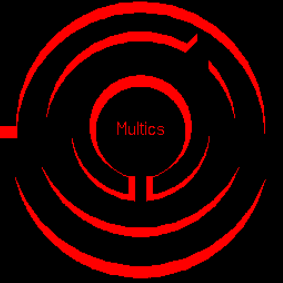
\includegraphics[width=.3\textwidth]{multics-logo}
			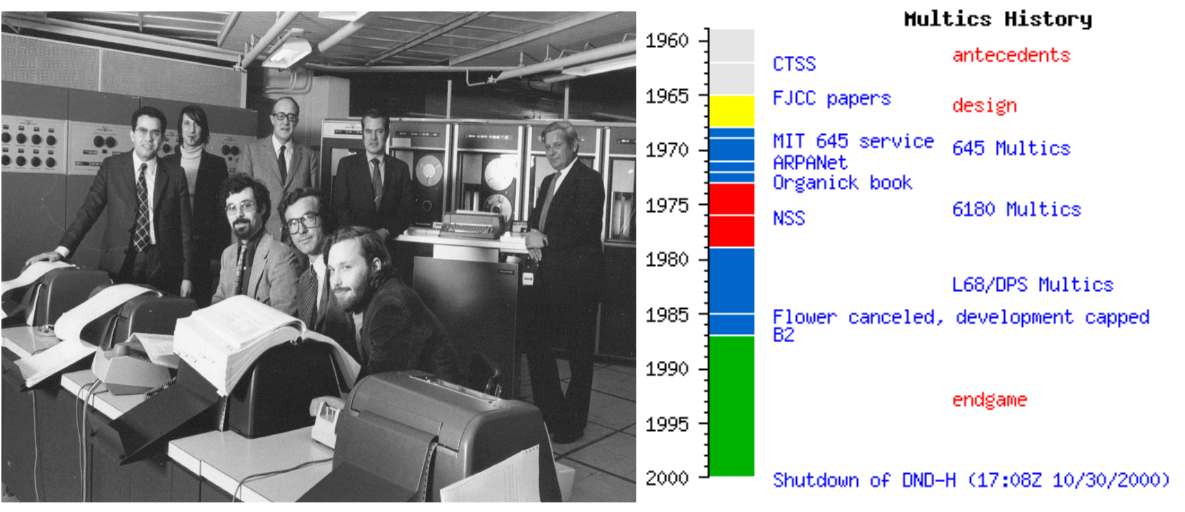
\includegraphics[width=1.\textwidth]{history-multics}


			
		\end{column}
		
		\begin{column}{.5\textwidth}
			
			\large
			MULTiplexed Information and Computing Service (MULTICS)
			\begin{itemize}
				\item Multics is a timesharing OS begun in 1964
				and used until 2000.
				
				\item  Joint project between MIT, Bell Labs, and GE
				
				\item  Primary usage was with a mainframe and
				multiple terminals.
				
%				\item CPUs, memory, I/O controllers, disk drives
%				could be added or removed while the
%				system is running

			\end{itemize}	
			
%			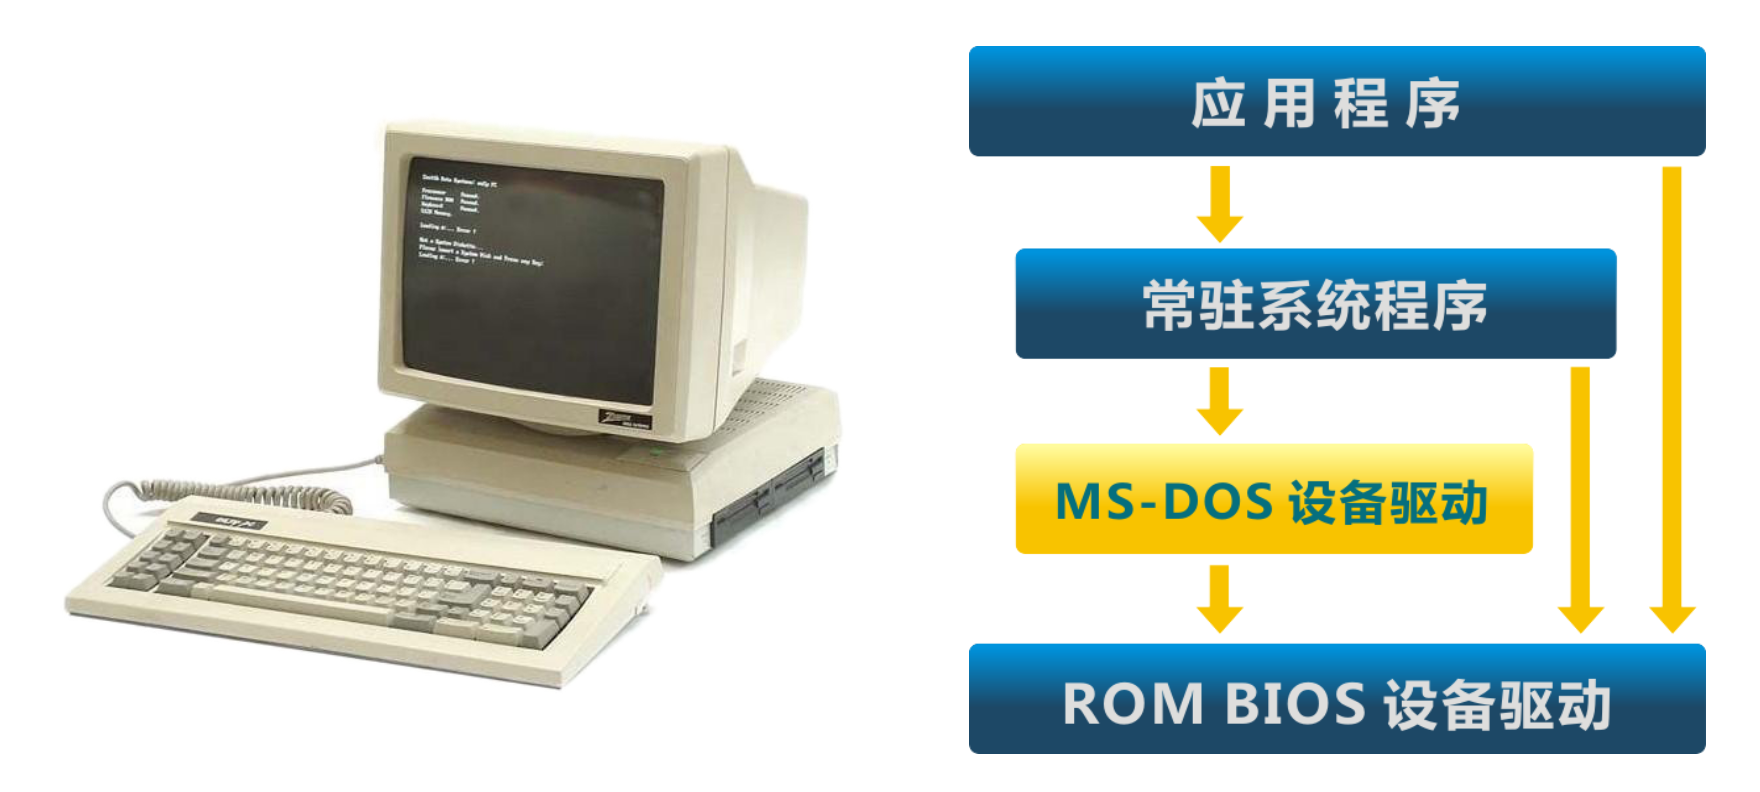
\includegraphics[width=1.\textwidth]{msdos}		
		\end{column}
		
		
	\end{columns}
	
	
\end{frame}

%-------------------------------------------------
\begin{frame}[plain]
	\frametitle{History}
	
	
	
	\begin{columns}
		
		\begin{column}{.5\textwidth}
			%			\centering
			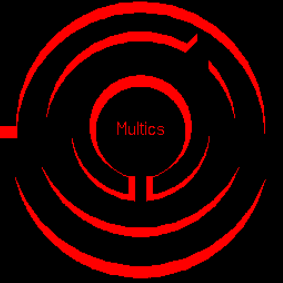
\includegraphics[width=.3\textwidth]{multics-logo}
			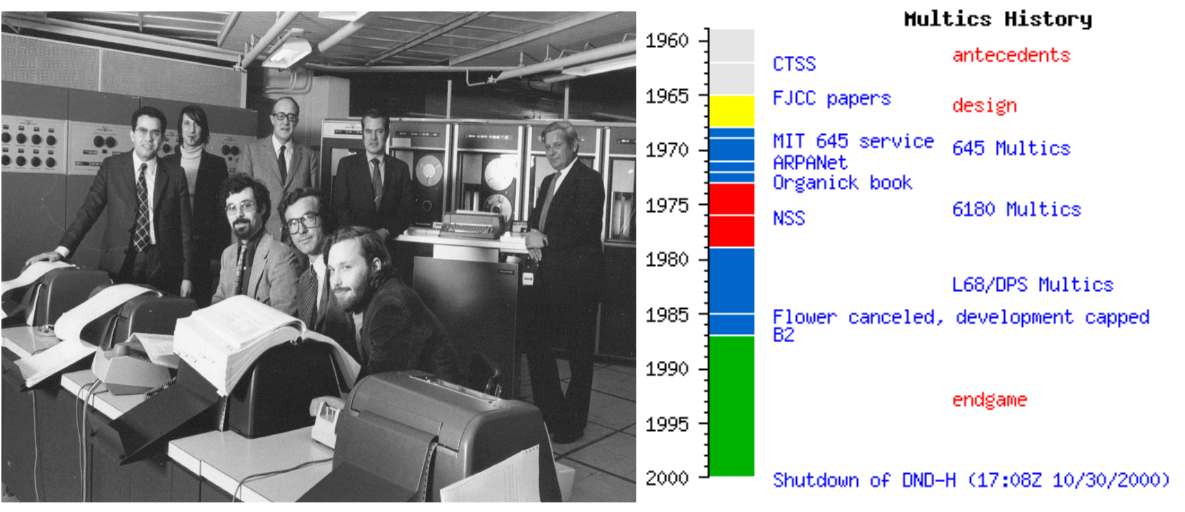
\includegraphics[width=1.\textwidth]{history-multics}
			
			
			
		\end{column}
		
		\begin{column}{.5\textwidth}
			
			\large
			Design Goals\&Features of  multics(1964) ?
			\begin{itemize}
				\item Segmented|Paging based Virtual memory
%Divided into as many as 2^14 segments
%Each segment has as many as 218 36-bit
%words
%Each segment is a logical unit of
%information with attributes for length and
%access privilege

% Main types of segments : Procedure, Data

				
				\item First hierarchical file system
				
%The term "file" and "segment" are often used
%interchangeably as a result of this one-to-one
%binding.

				
				\item High-level language implementation (IBM's PL/I)
%				 In 1965 this was a new proposal by IBM
%			  	 Only a small part of the OS was written in assembly
%				 Writing an OS in a high-level language
%				was a radical idea at the time
				
				\item Shared memory multiprocessor
				\item Dynamic linking and function call by name
				\item Security and rings
			\end{itemize}	

		\end{column}
		
		
	\end{columns}
	
	
\end{frame}

%-------------------------------------------------
\begin{frame}[plain]
	\frametitle{History}
	
	
	
	\begin{columns}
		
		\begin{column}{.5\textwidth}
			%			\centering
			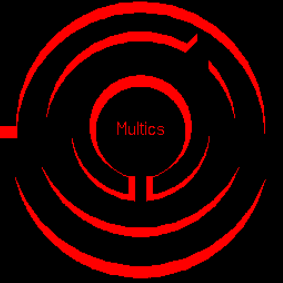
\includegraphics[width=.1\textwidth]{multics-logo}
			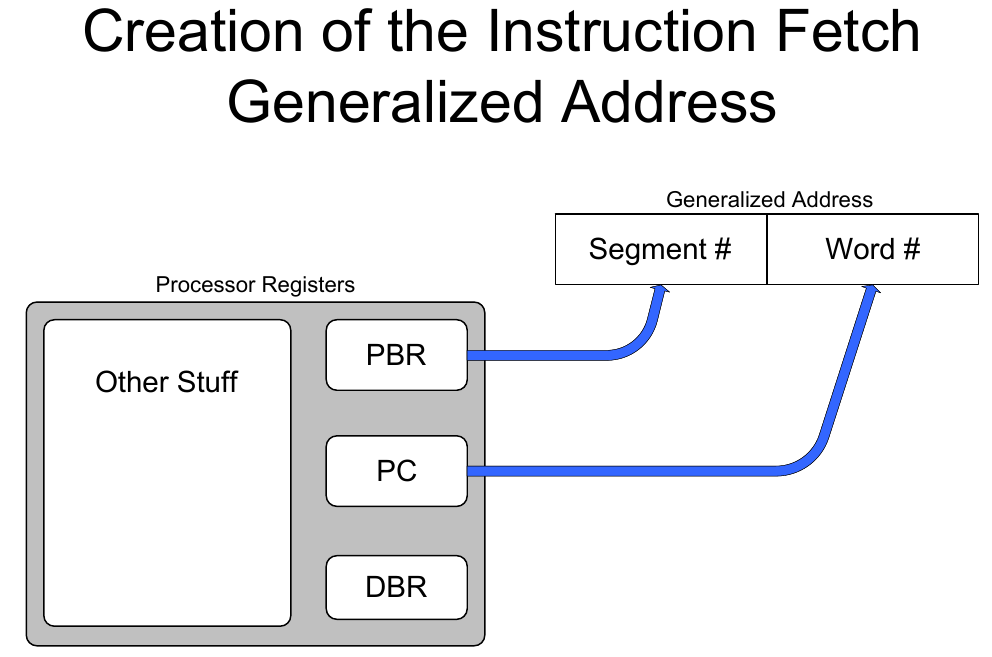
\includegraphics[width=1.\textwidth]{multics-intr-address}
			
			
			
		\end{column}
		
		\begin{column}{.5\textwidth}
			
			\Large
			Addressing
			\begin{itemize}
				\item  Multics uses a	“Generalized Address”
				\item  It is calculated
				differently depending
				on if the CPU is
				attempting to read an
				instruction or data

				
			\end{itemize}	
			
			%			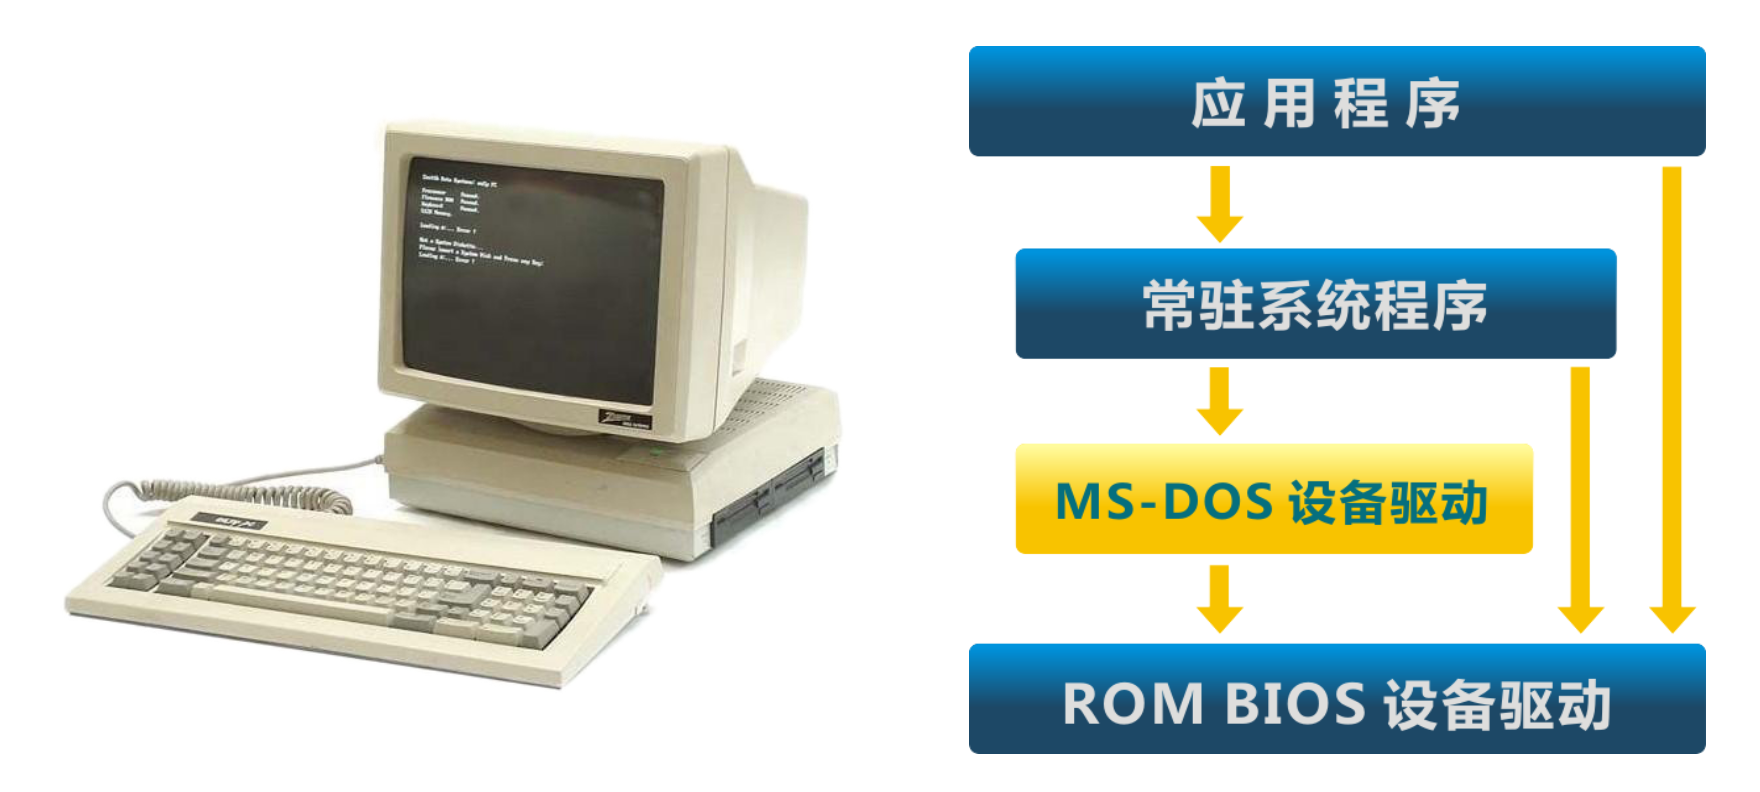
\includegraphics[width=1.\textwidth]{msdos}		
		\end{column}
		
		
	\end{columns}
	
	
\end{frame}


%-------------------------------------------------
\begin{frame}[plain]
	\frametitle{History}
	
	
	
	\begin{columns}
		
		\begin{column}{.5\textwidth}
			%			\centering
			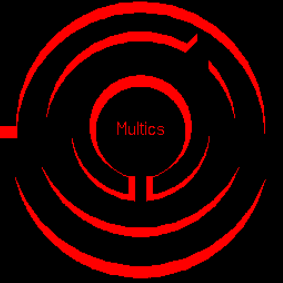
\includegraphics[width=.1\textwidth]{multics-logo}
			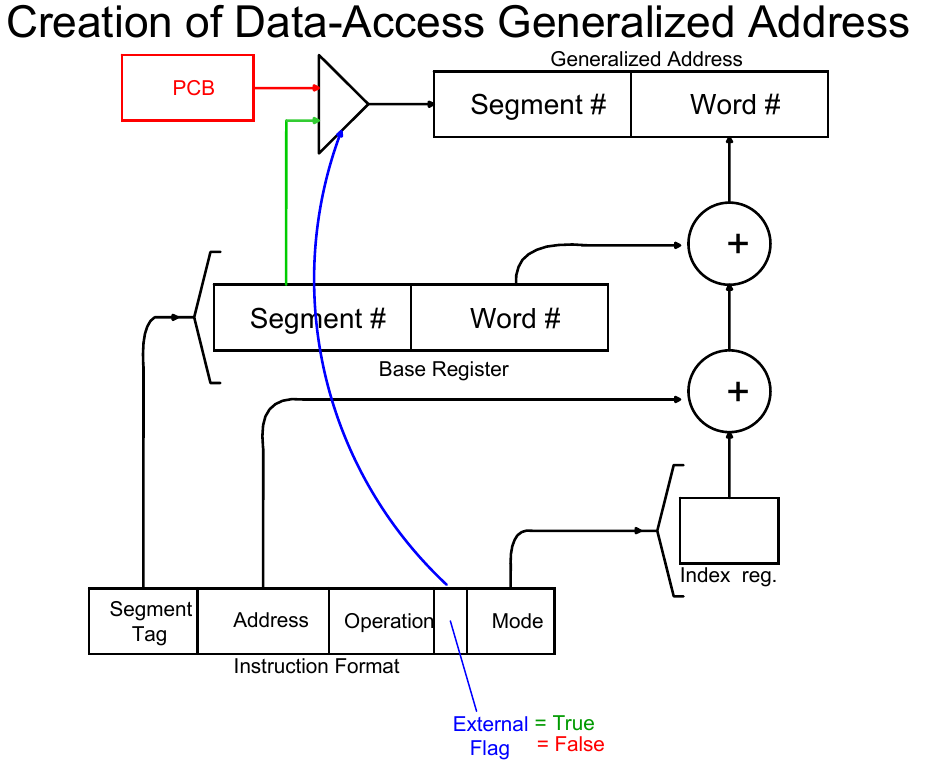
\includegraphics[width=1.\textwidth]{multics-data-address}
			
			
			
		\end{column}
		
		\begin{column}{.5\textwidth}
			
			\Large
			Addressing
			\begin{itemize}
				\item  Multics uses a “Generalized Address”
				\item  It is calculated
				differently depending
				on if the CPU is
				attempting to read an
				instruction or data
				
				
			\end{itemize}	
			
			%			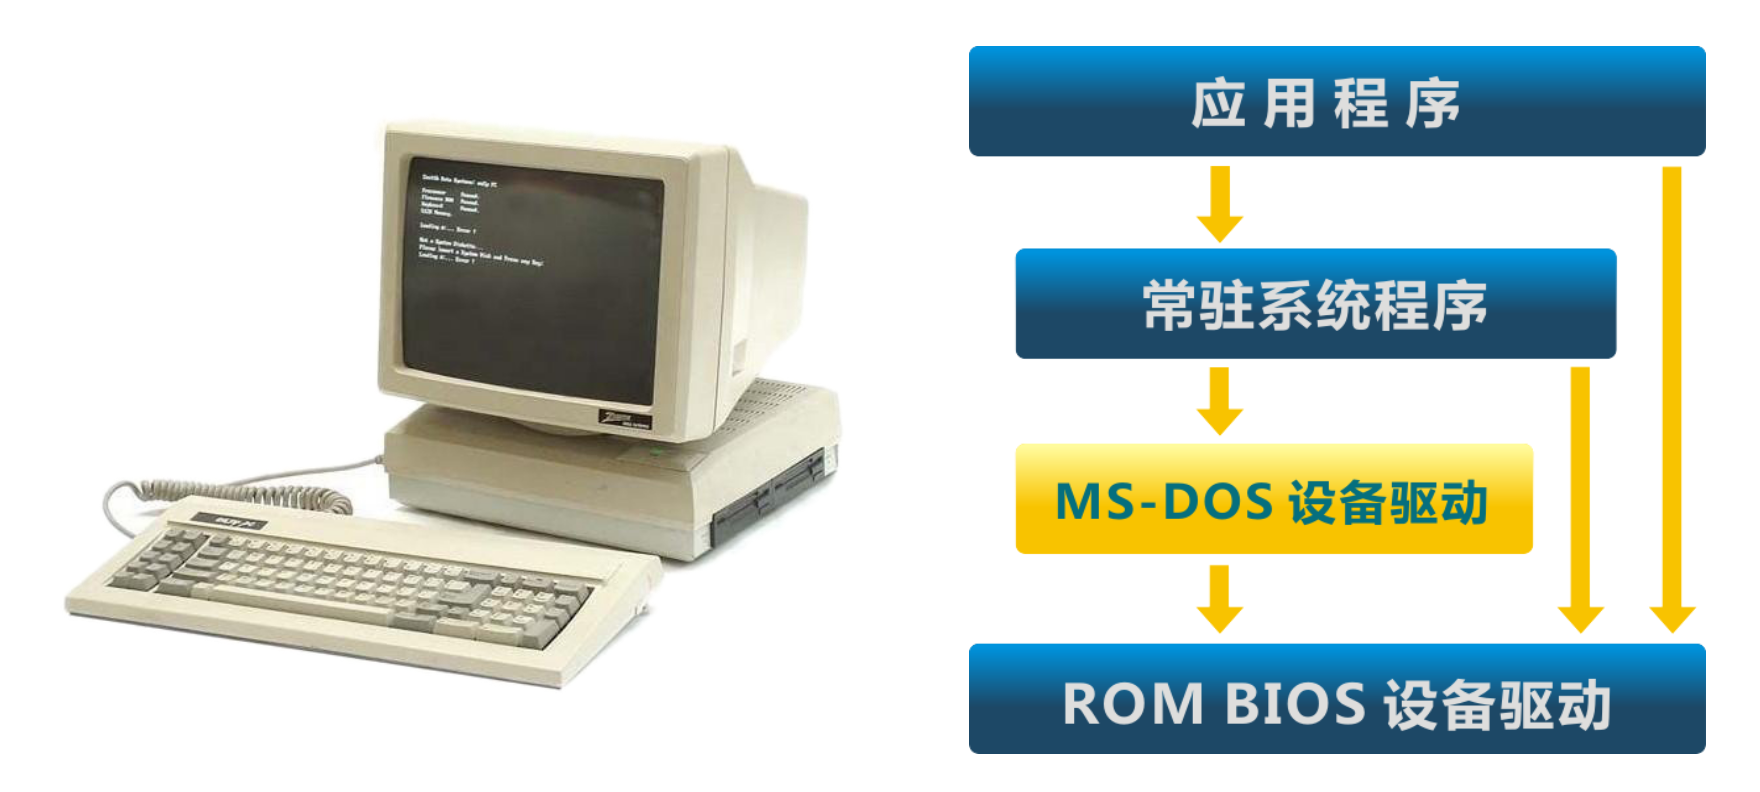
\includegraphics[width=1.\textwidth]{msdos}		
		\end{column}
		
		
	\end{columns}
	
	
\end{frame}
%-------------------------------------------------



%-------------------------------------------------
\begin{frame}[plain]
	\frametitle{History}
	
	
	
	\begin{columns}

		\begin{column}{.4\textwidth}
			\centering
			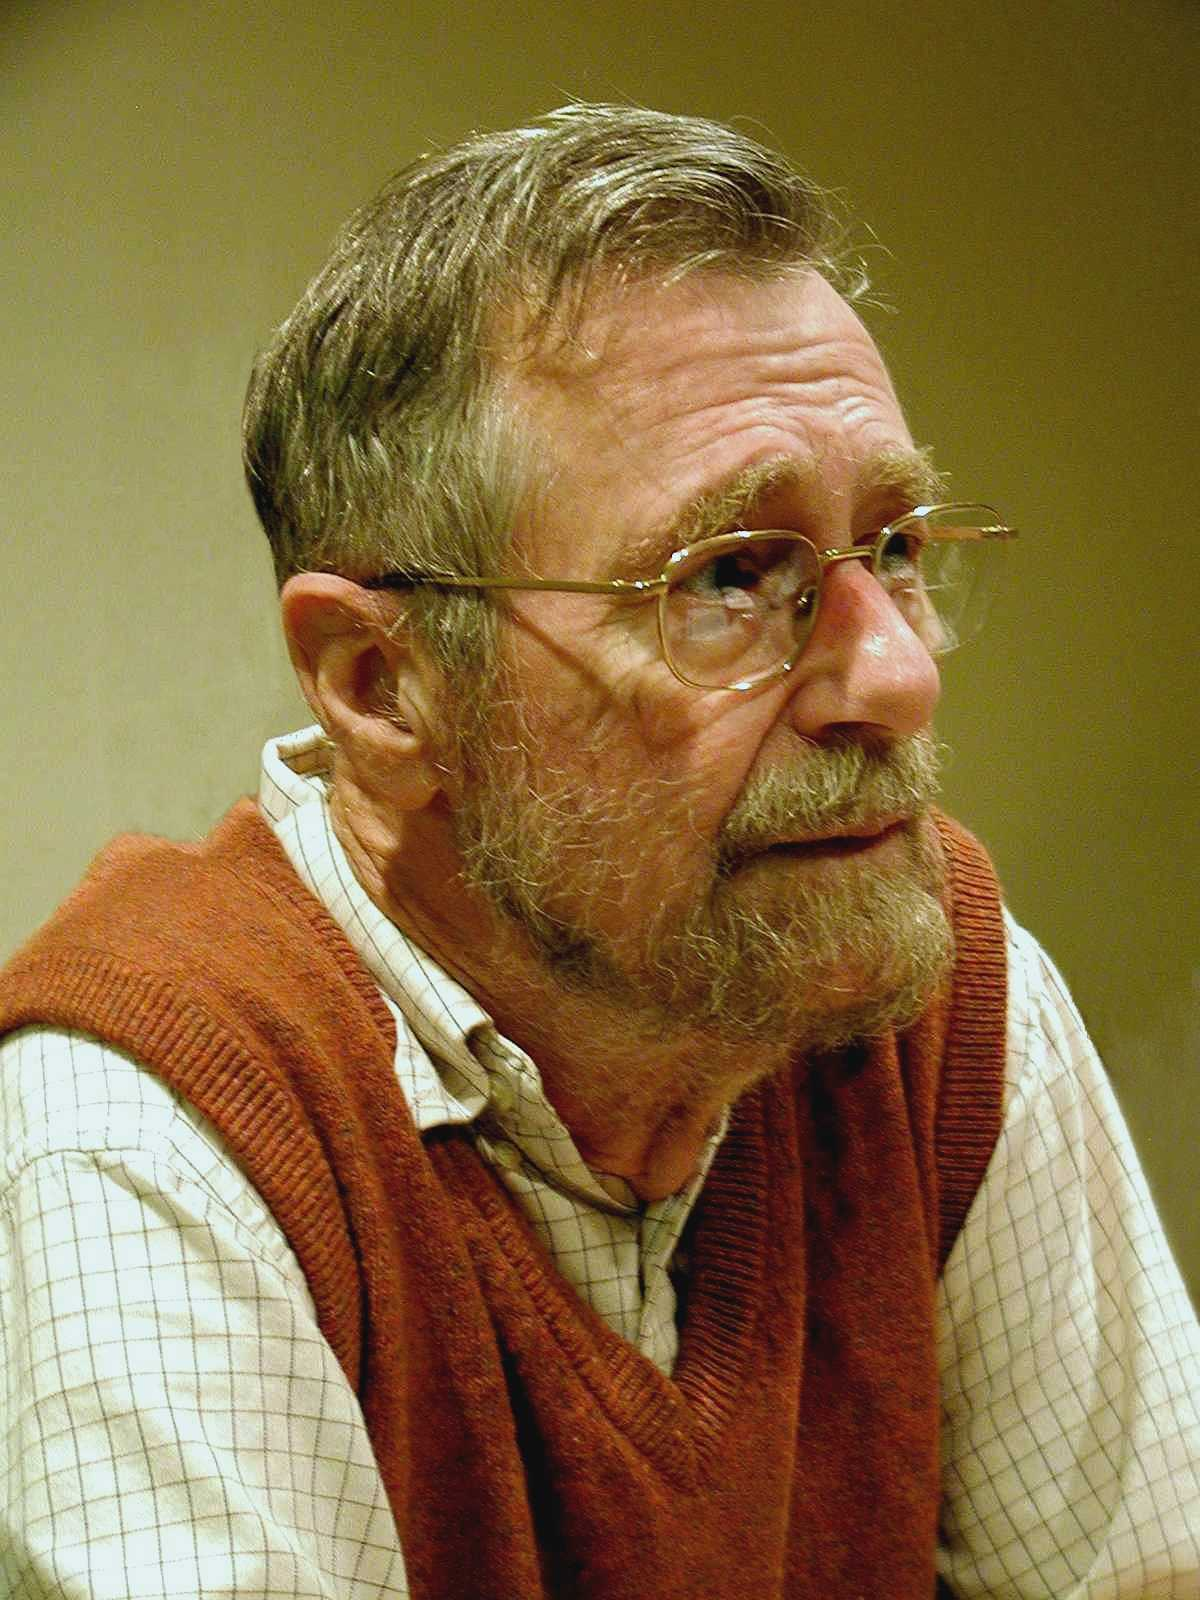
\includegraphics[width=.3\textwidth]{EWD}
			
\includegraphics[width=1.\textwidth]{harmful-goto}
			
			
			
		\end{column}
		
		\begin{column}{.6\textwidth}
			
%			\large
			The Structure of the “The” - Multiprogramming System
			\begin{itemize}
				\item May, 1968
				
				\item  Response to a call for papers on timely research and development efforts
				
				\item  Six person team

				\item  3 Guiding Principles
					\begin{itemize}
					\item Select an ambitious project
					\item Select a machine with a good basic design (EL X8)
%					32K core memory
%					512K words drum size
%					Good peripheral and interrupt control
%					Several low capacity channels
%					Tape readers/writers, printers, etc
%					Lack of other awkward features
					\item Experience != Wisdom
					\end{itemize}
					
				\end{itemize}	
					
			\end{column}

	\end{columns}


\end{frame}

%--------------------%-------------------------------------------------
\begin{frame}[plain]
	\frametitle{History}
	
	
	
	\begin{columns}
		
		\begin{column}{.4\textwidth}
			\centering
			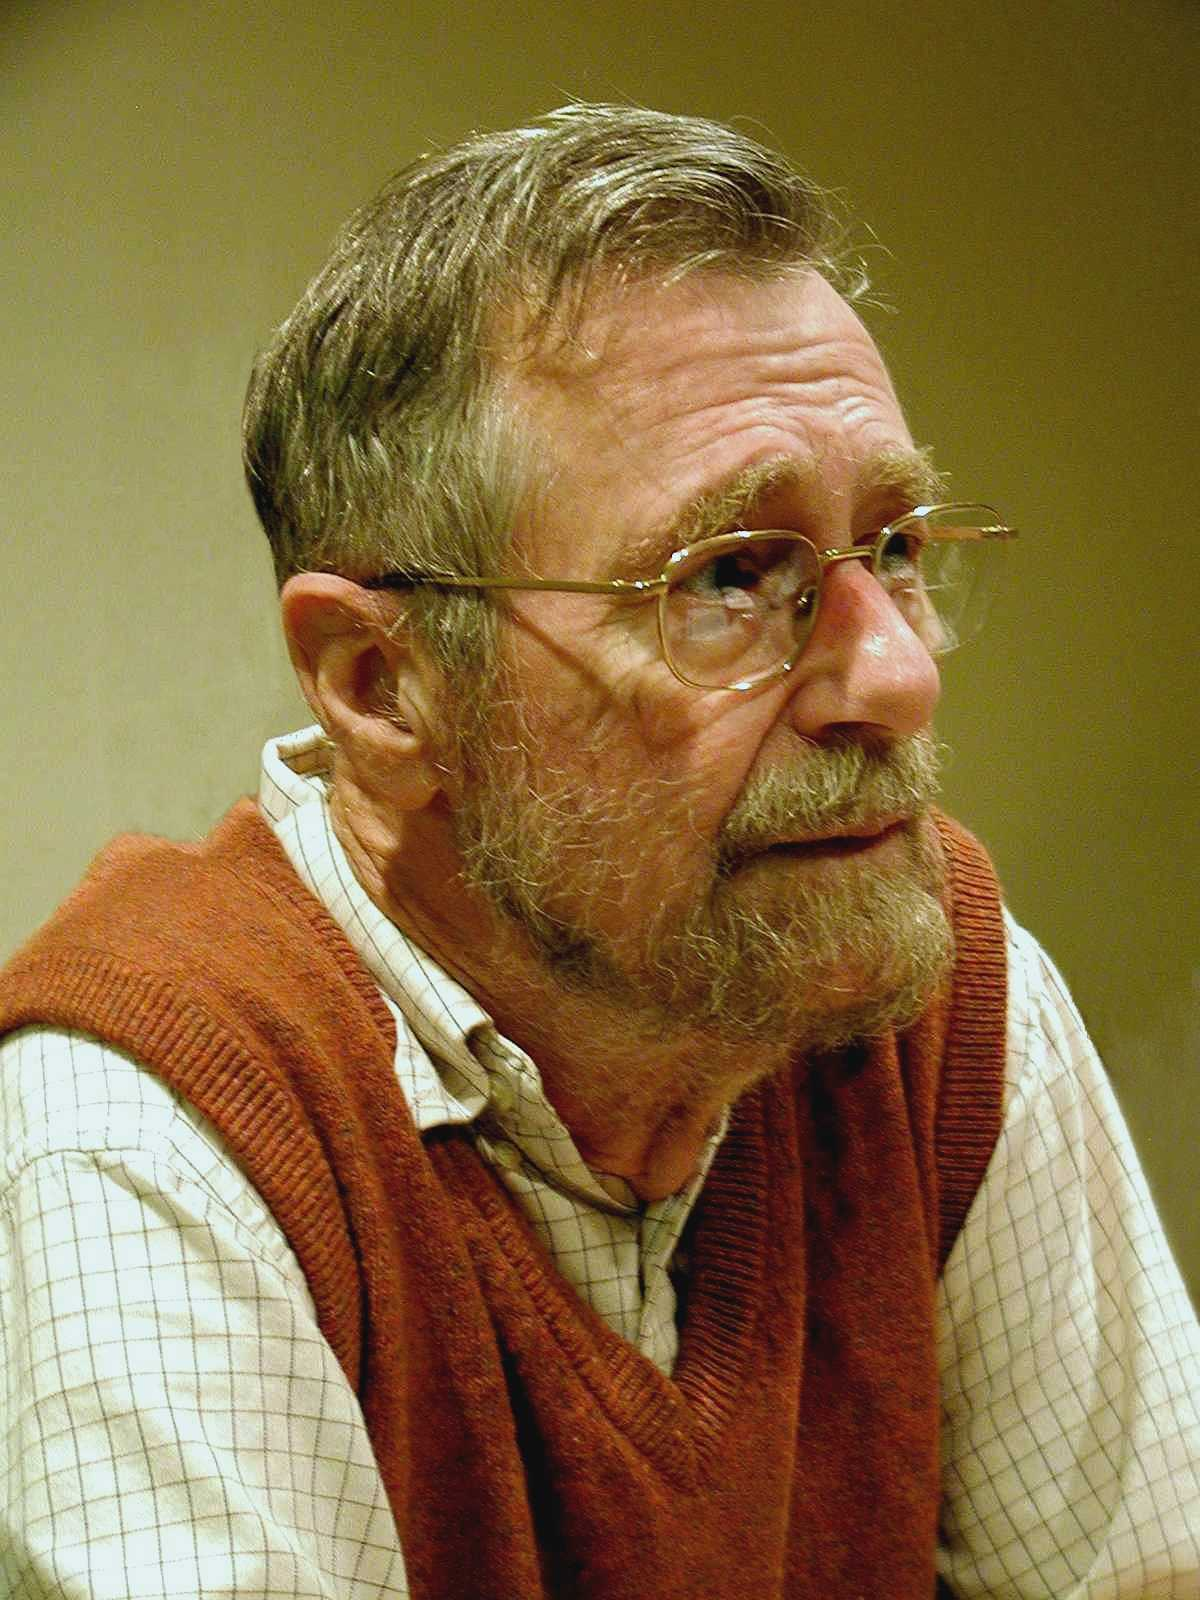
\includegraphics[width=.3\textwidth]{EWD}
			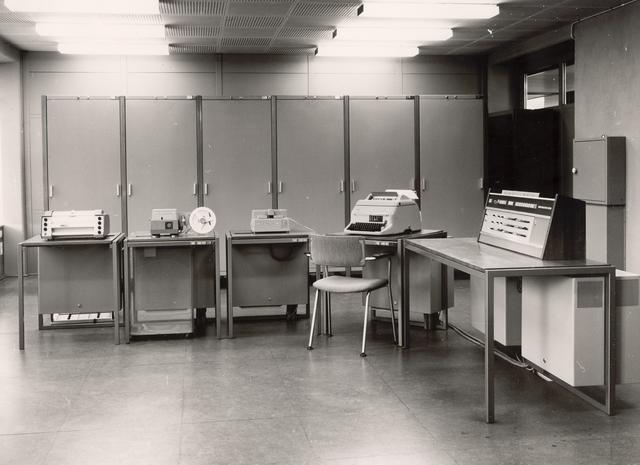
\includegraphics[width=1.\textwidth]{elx8}
			
			
			
		\end{column}
		
		\begin{column}{.6\textwidth}
			
%	\large
	\begin{block}{SIGOPS Hall of Fame summary}
“The first paper to suggest that an operating system be built in a structured way. That structure was a series of layers, each a virtual machine that introduced abstractions built using the functionality of lower layers. The paper stimulated a great deal of subsequent work in building operating systems as structured systems.”
\end{block} 
	\large
	\begin{itemize}
	\item Contributions
	\begin{itemize}
		\item System Hierarchy					
		\item Storage Allocation
		\item Processor Allocation
		
		\item Semaphores
		
	\end{itemize}
	
\end{itemize}	
			
		\end{column}
		
		
	\end{columns}
	
	
\end{frame}

%-------------------------------------------------


\begin{frame}[plain]
	\frametitle{History}
	
	
	
	\begin{columns}
		
		\begin{column}{.4\textwidth}
			\centering
			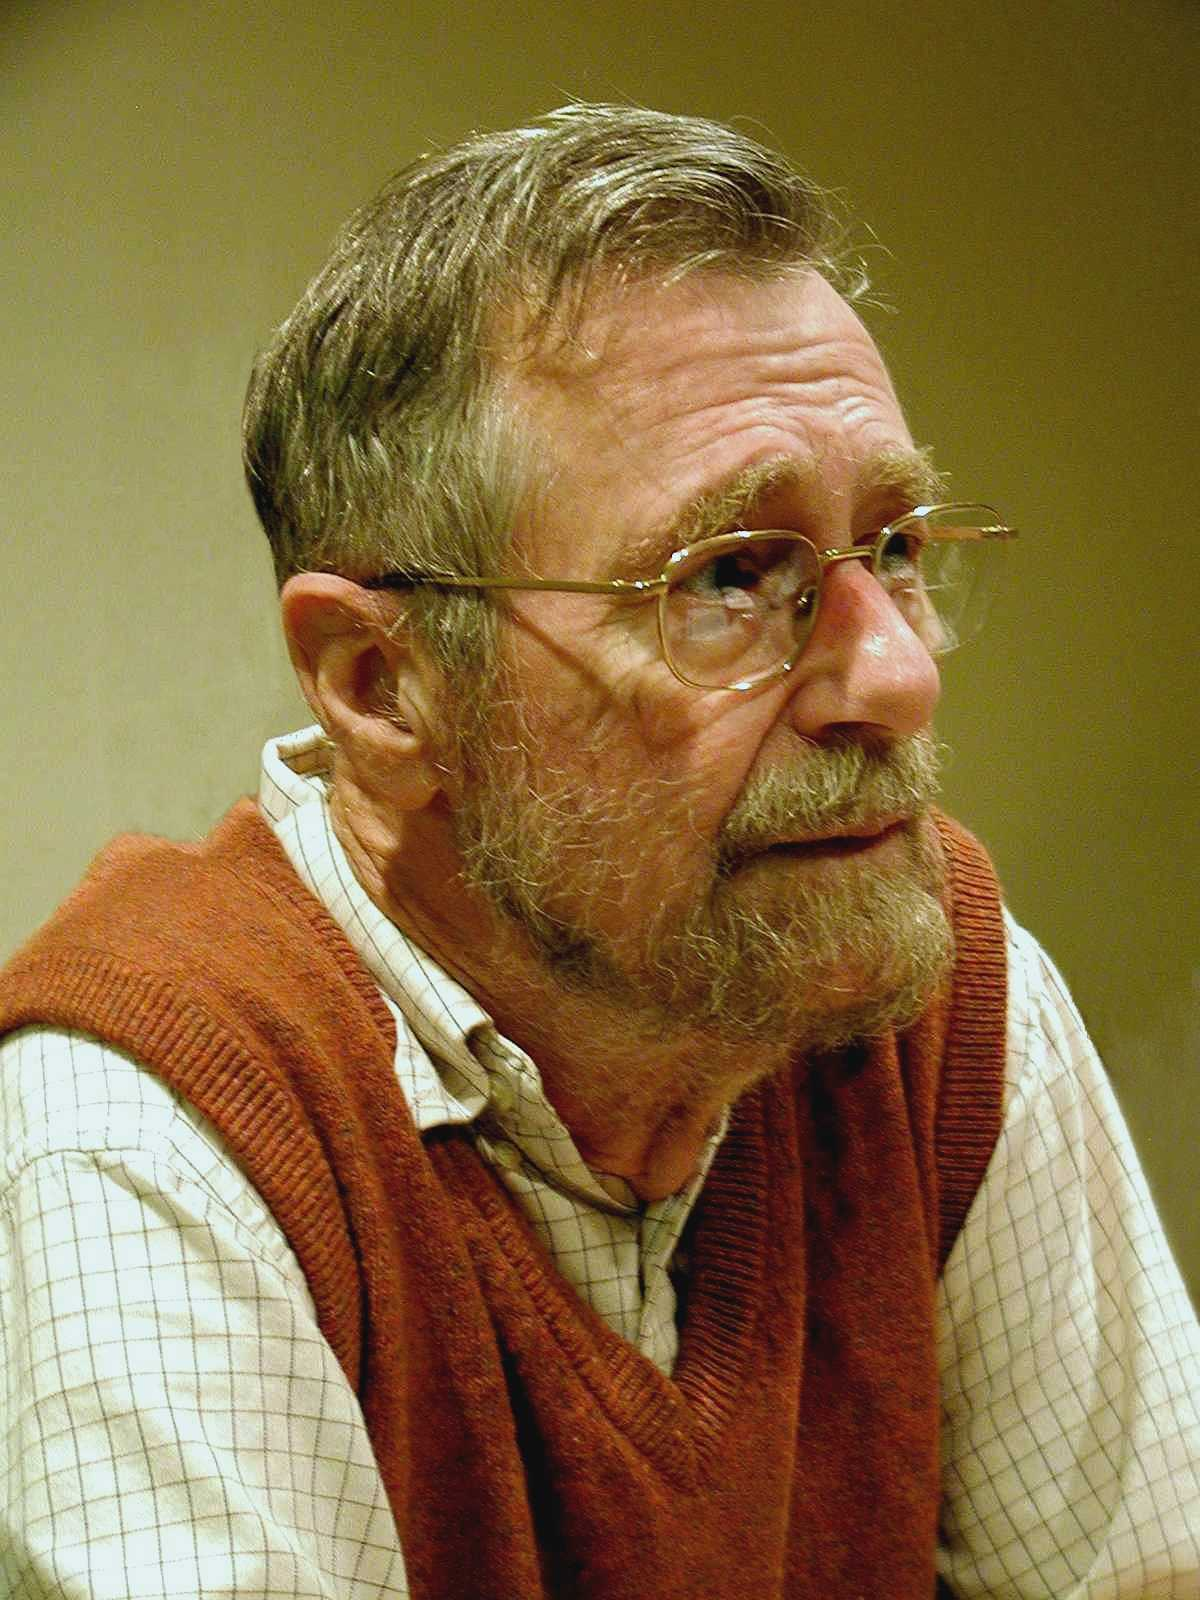
\includegraphics[width=.3\textwidth]{EWD}
			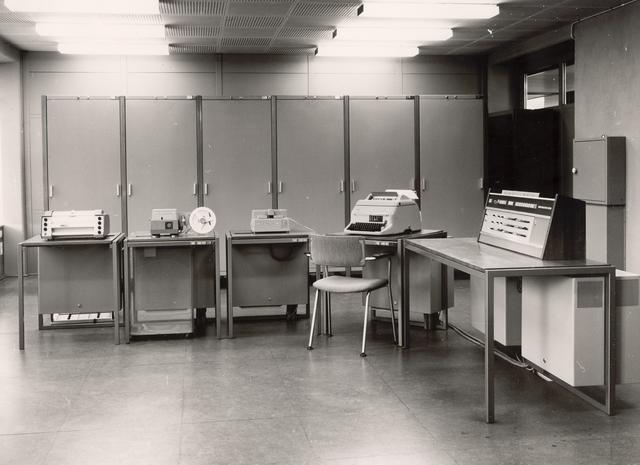
\includegraphics[width=1.\textwidth]{elx8}
			
			
			
		\end{column}
		
		\begin{column}{.6\textwidth}
			
			%			\large
			The Structure of the “The” - Multiprogramming System
			\begin{itemize}
				\item Contributions
				\begin{itemize}
					\item System Hierarchy					
					\item Storage Allocation
					\item Processor Allocation

					\item Semaphores
					
				\end{itemize}
				
			\end{itemize}	
			
		\end{column}
		
		
	\end{columns}
	
	
\end{frame}



%-------------------------------------------------
\begin{frame}[plain]
	\frametitle{History}
	
	
	
	\begin{columns}
		
		\begin{column}{.4\textwidth}
			\centering
			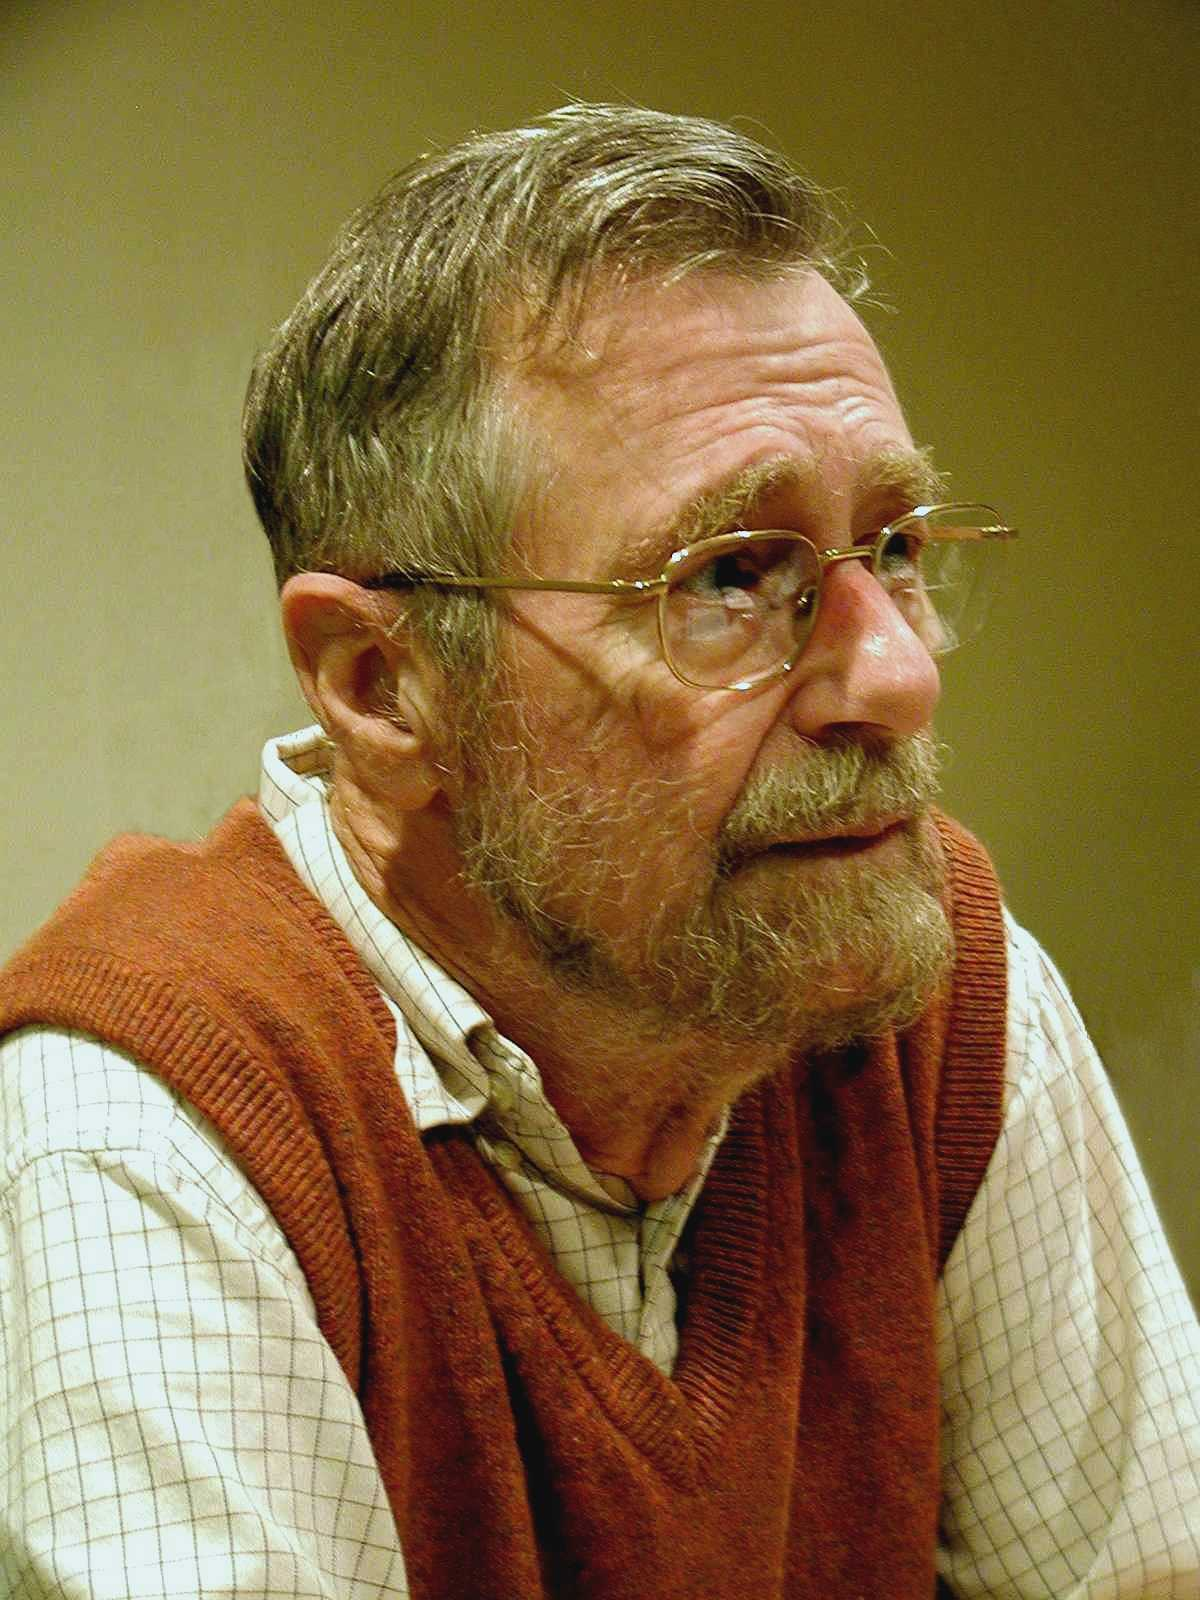
\includegraphics[width=.3\textwidth]{EWD}
			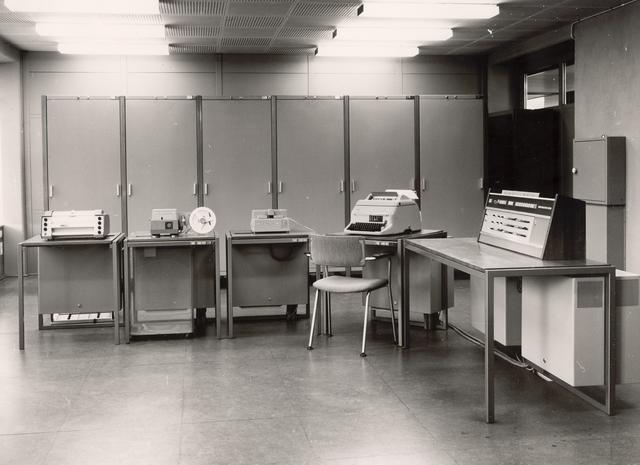
\includegraphics[width=1.\textwidth]{elx8}
			
			
			
		\end{column}
		
		\begin{column}{.6\textwidth}
			
			%			\large
			The Structure of the “The” - Multiprogramming System
			\begin{itemize}
				\item Goal
				\begin{itemize}
					\item Quick turn-around for short term programs
					\item Economic peripheral use
					\item Economic backing store and processor use
					\item Flexibility as a general purpose computer
				\end{itemize}
				
			\end{itemize}	
			
		\end{column}
		
		
	\end{columns}
	
	
\end{frame}


%-------------------------------------------------
\begin{frame}[plain]
	\frametitle{History}
	
	
	
	\begin{columns}
		
		\begin{column}{.4\textwidth}
			\centering
			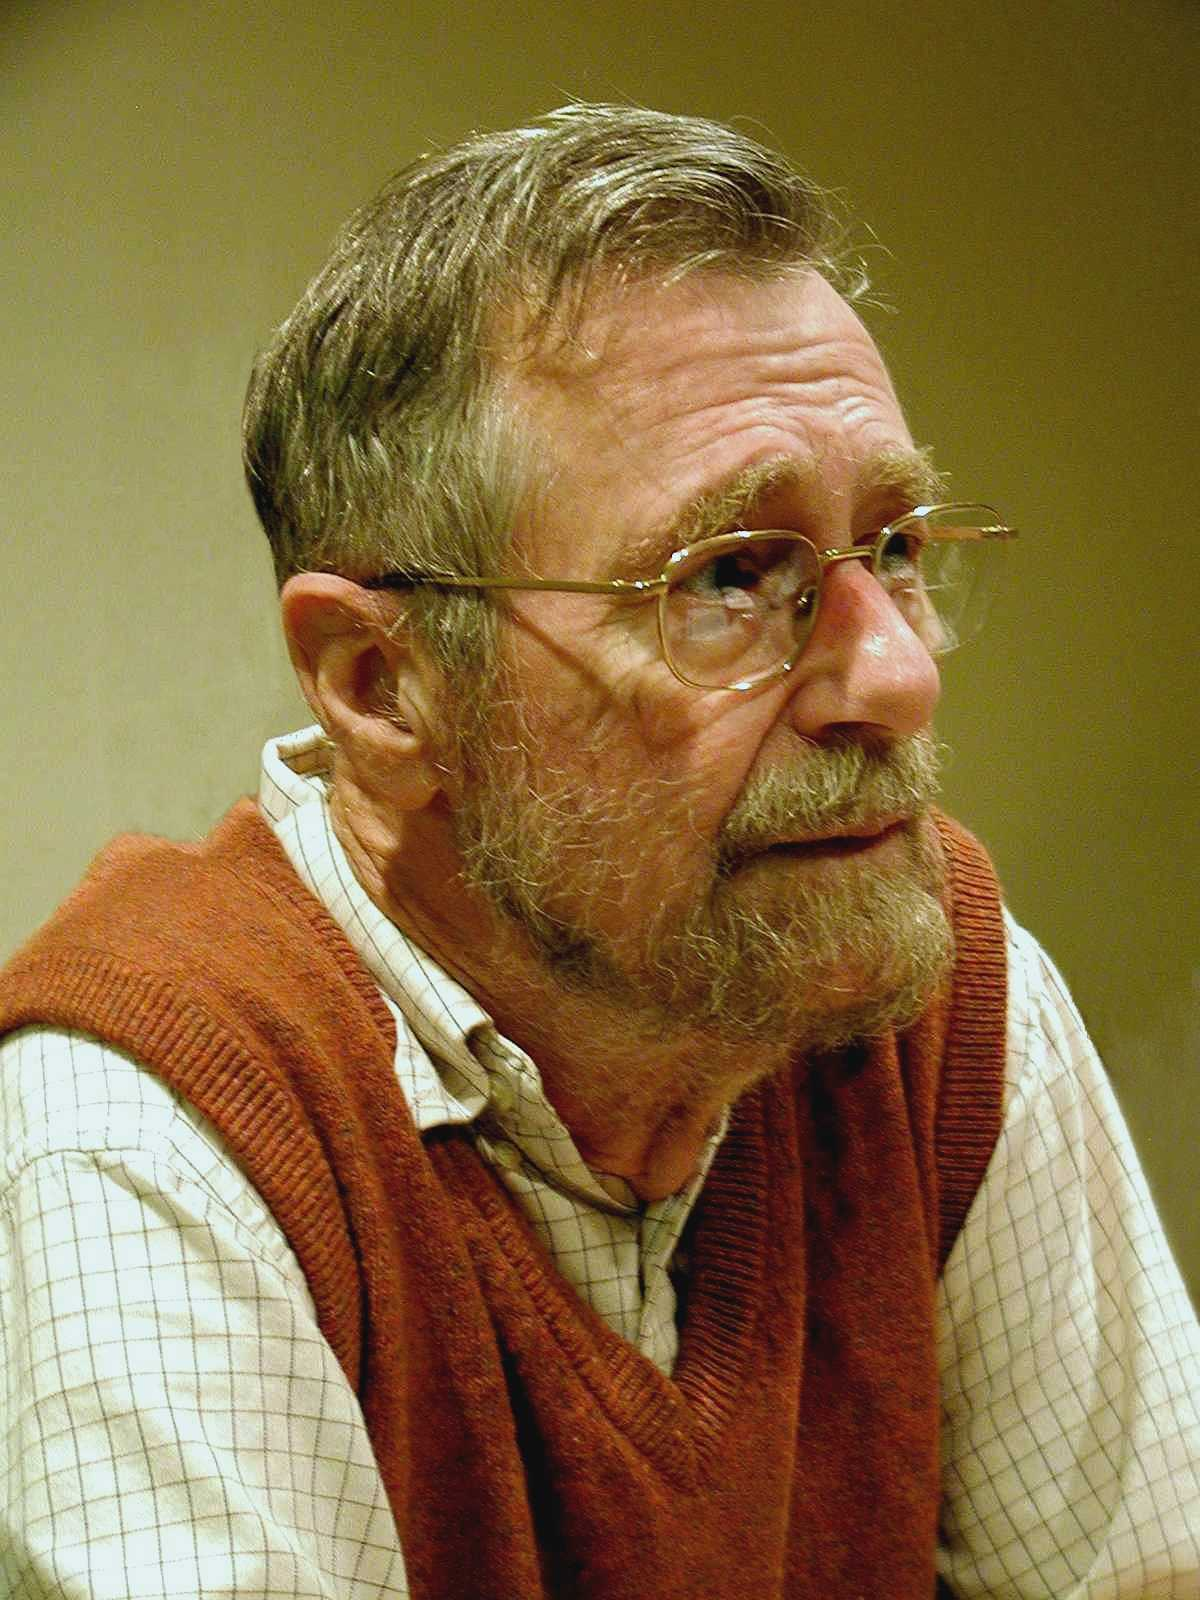
\includegraphics[width=.3\textwidth]{EWD}
			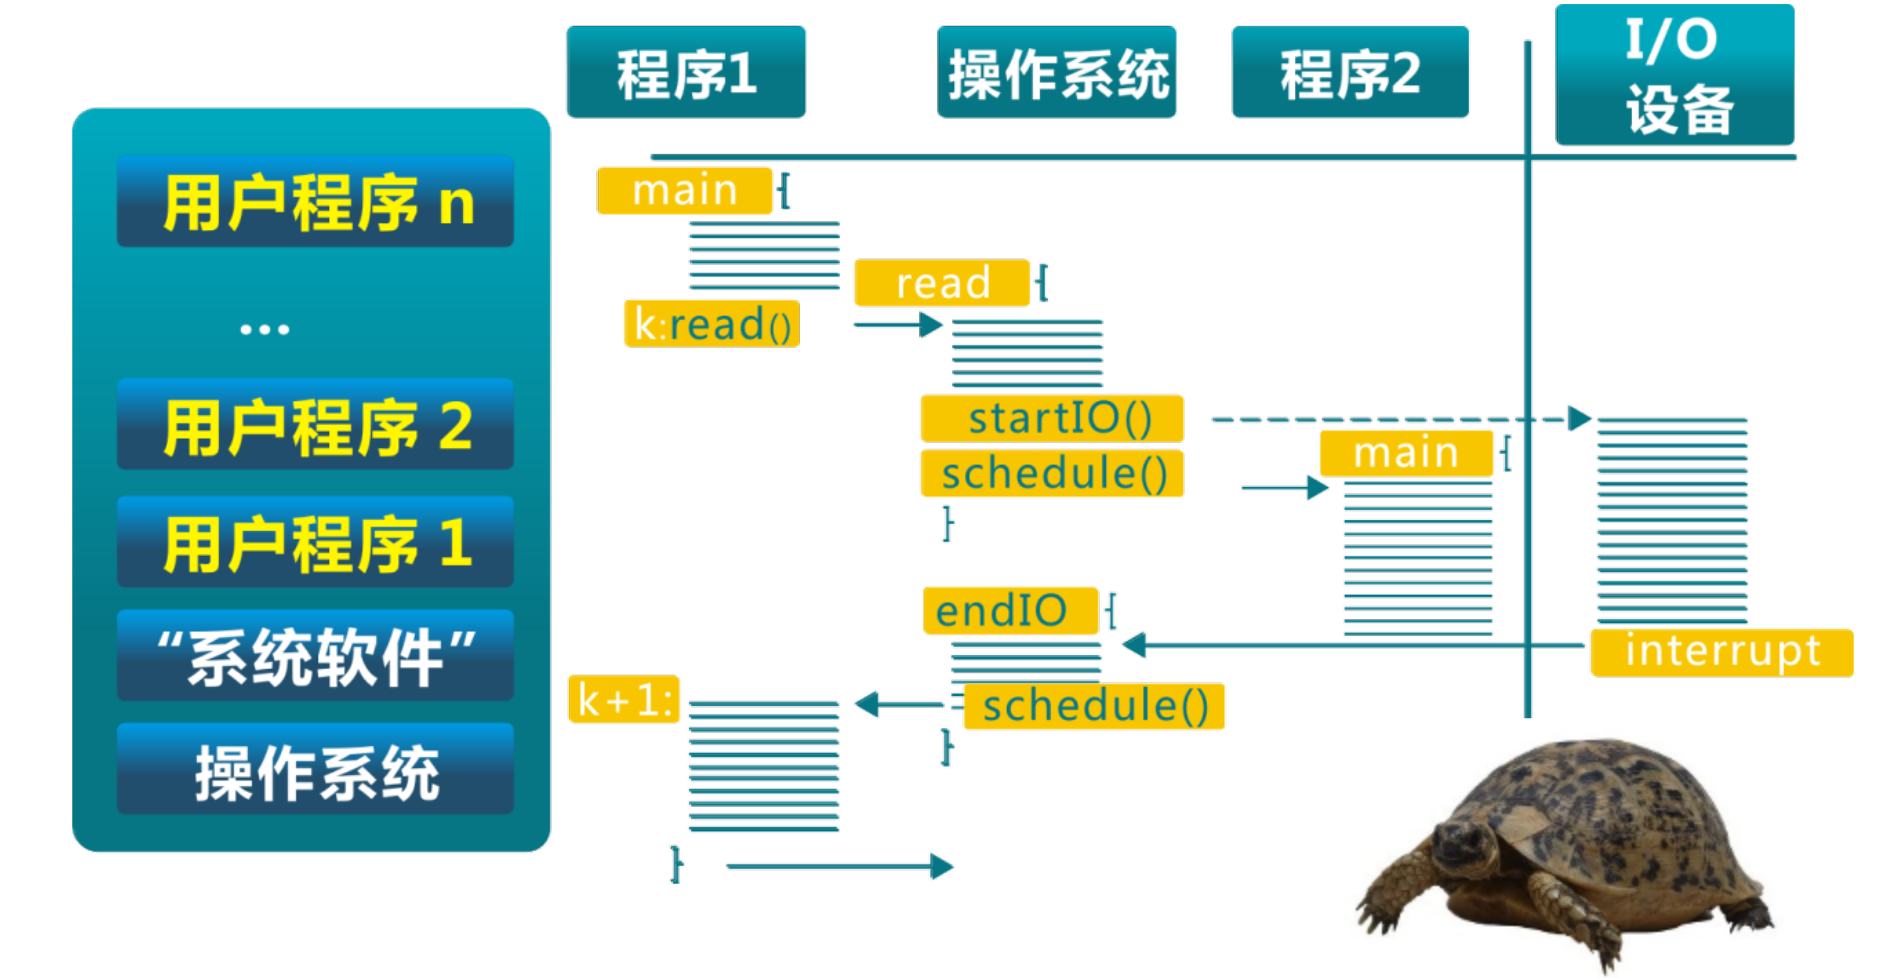
\includegraphics[width=1.\textwidth]{multiprogramming}
			
			
			
		\end{column}
		
		\begin{column}{.6\textwidth}
			
			%			\large
			The Structure of the “The” - Multiprogramming System
			\begin{itemize}
				\item Challenge : Multiprogramming
				\item Challenge : Complex softwares v.s. puny hardware
				
			\end{itemize}	
			
		\end{column}
		
		
	\end{columns}
	
	
\end{frame}


%-------------------------------------------------
\begin{frame}[plain]
	\frametitle{History}
	
	
	
	\begin{columns}
		
		\begin{column}{.4\textwidth}
			\centering
			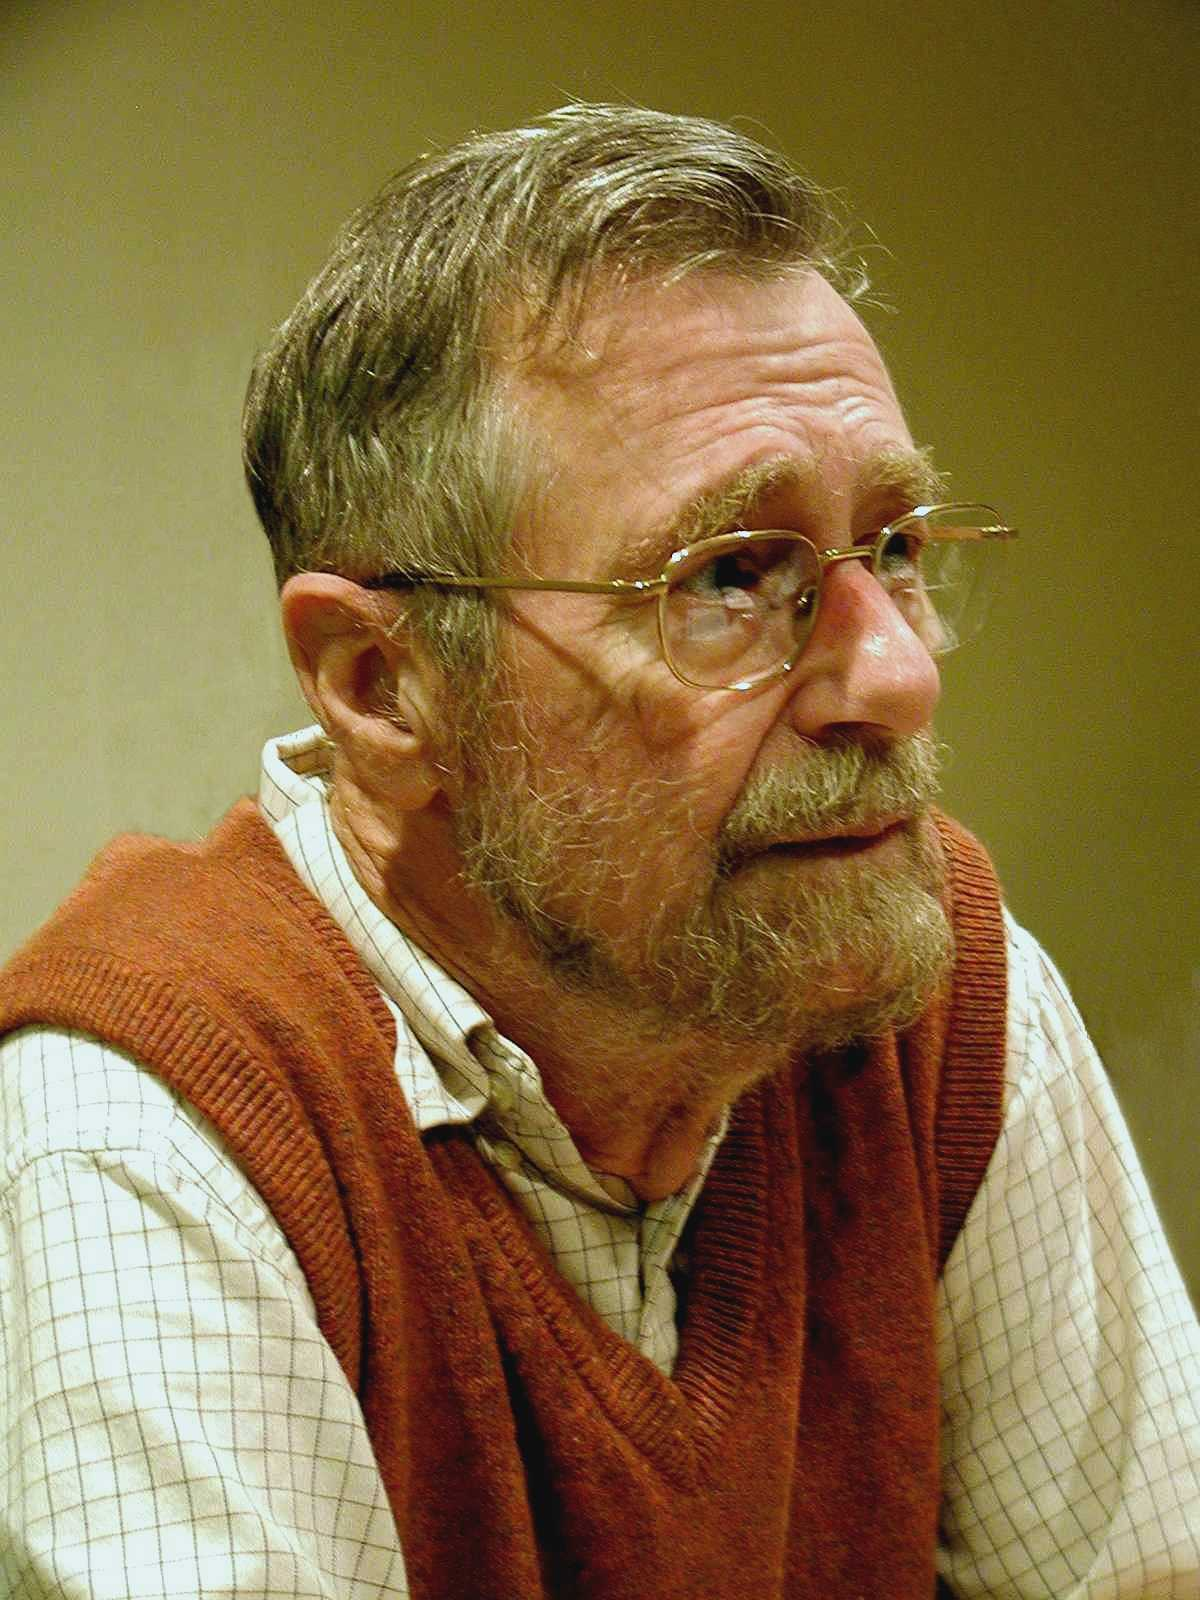
\includegraphics[width=.2\textwidth]{EWD}
			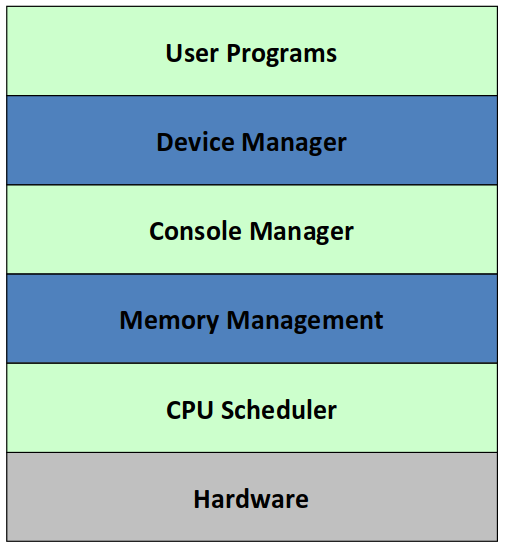
\includegraphics[width=.8\textwidth]{THE-layered-structure}
			
			
			
		\end{column}
		
		\begin{column}{.6\textwidth}
			
			%			\large
			The Structure of the “The” - Multiprogramming System
			\begin{itemize}
				\item Solution : Layered Structure
				
				\begin{itemize}
					\item Virtualized i/o streams
					\item Private console
					\item One huge/unlimited memory space
					\item One processor, manage interrupt
				\end{itemize}
				
			\end{itemize}	
			
		\end{column}
		
		
	\end{columns}
	
	
\end{frame}


%-------------------------------------------------
\begin{frame}[plain]
	\frametitle{History}
	
	
	
	\begin{columns}
		
		\begin{column}{.4\textwidth}
			\centering
			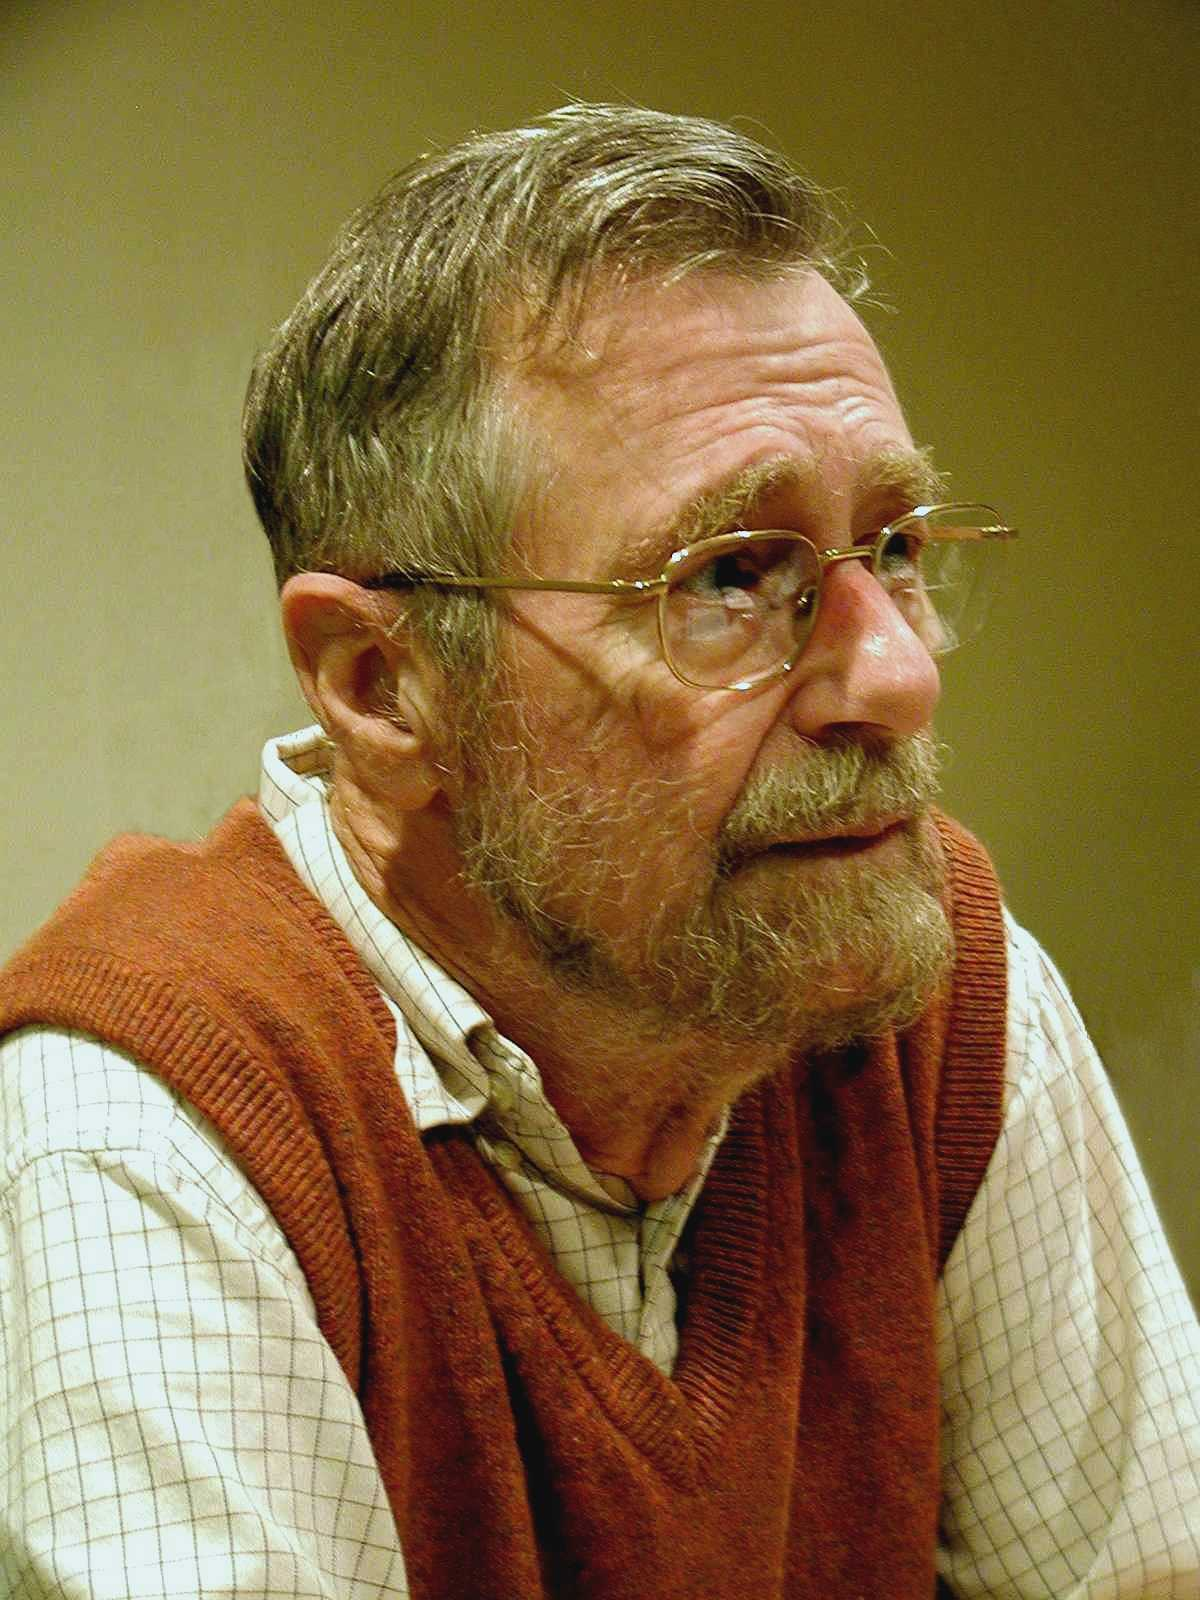
\includegraphics[width=.2\textwidth]{EWD}
			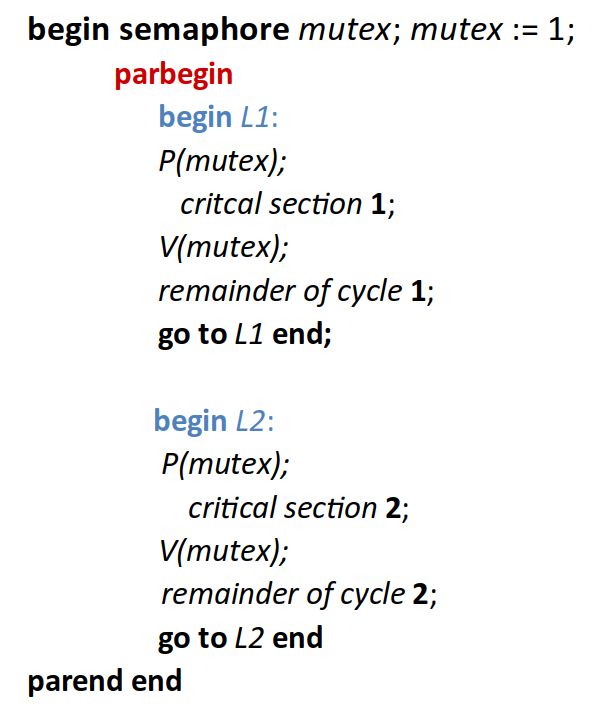
\includegraphics[width=.8\textwidth]{semaphore}
			
			
			
		\end{column}
		
		\begin{column}{.6\textwidth}
			
			%			\large
			The Structure of the “The” - Multiprogramming System
			\begin{itemize}
				\item Solution : Semaphore
				
				\begin{itemize}
					\item The OS requires synchronization

				\end{itemize}
				
			\end{itemize}	
			
		\end{column}
		
		
	\end{columns}
	
	
\end{frame}


%-------------------------------------------------
\begin{frame}[plain]
	\frametitle{History}
	
	
	
	\begin{columns}
		
		\begin{column}{.4\textwidth}
			\centering
			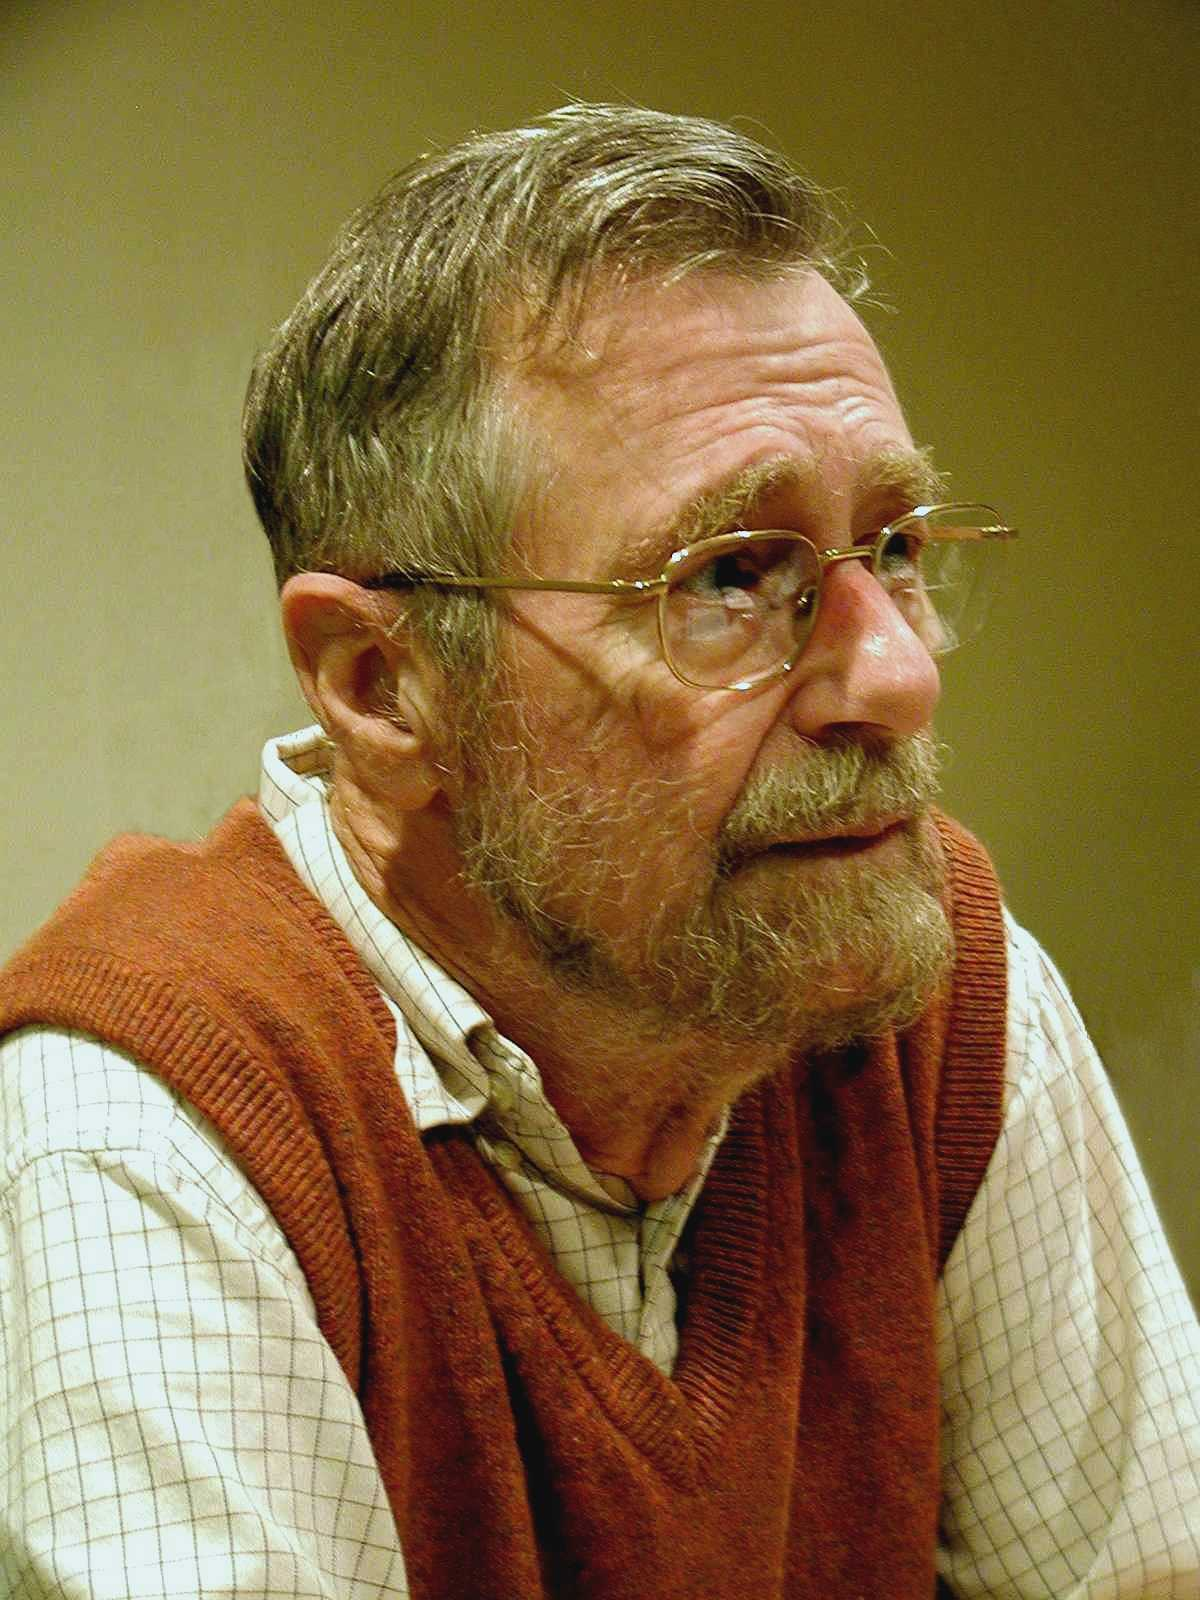
\includegraphics[width=.2\textwidth]{EWD}
			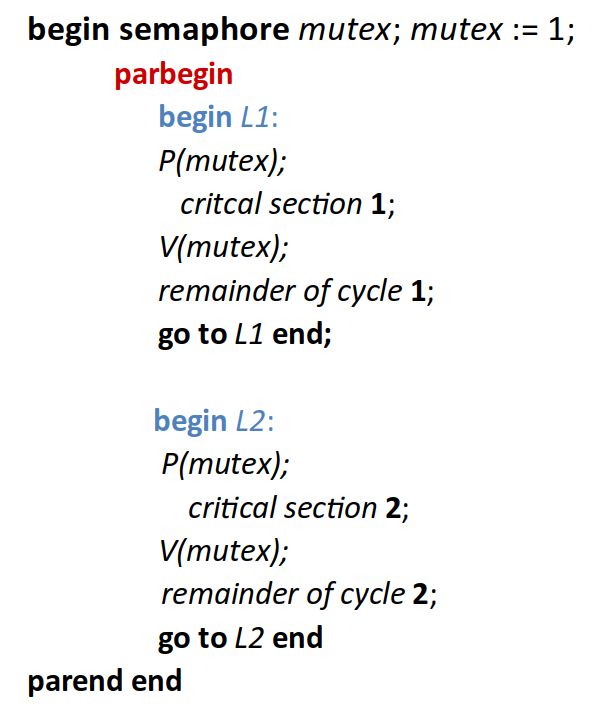
\includegraphics[width=.8\textwidth]{semaphore}
			
			
			
		\end{column}
		
		\begin{column}{.6\textwidth}
			
			%			\large
			The Structure of the “The” - Multiprogramming System
			\begin{itemize}
				\item Future : verification
				
				\begin{itemize}
					\item Testing was done from the bottom level up, Each level was exhaustively tested prior to the next. But Testing is not enough.
					
				\end{itemize}
				
			\end{itemize}	
			
		\end{column}
		
		
	\end{columns}
	
	
\end{frame}


%-------------------------------------------------
\begin{frame}[plain]
	\frametitle{History}
	
	
	
	\begin{columns}
		
		\begin{column}{.4\textwidth}
			\centering
			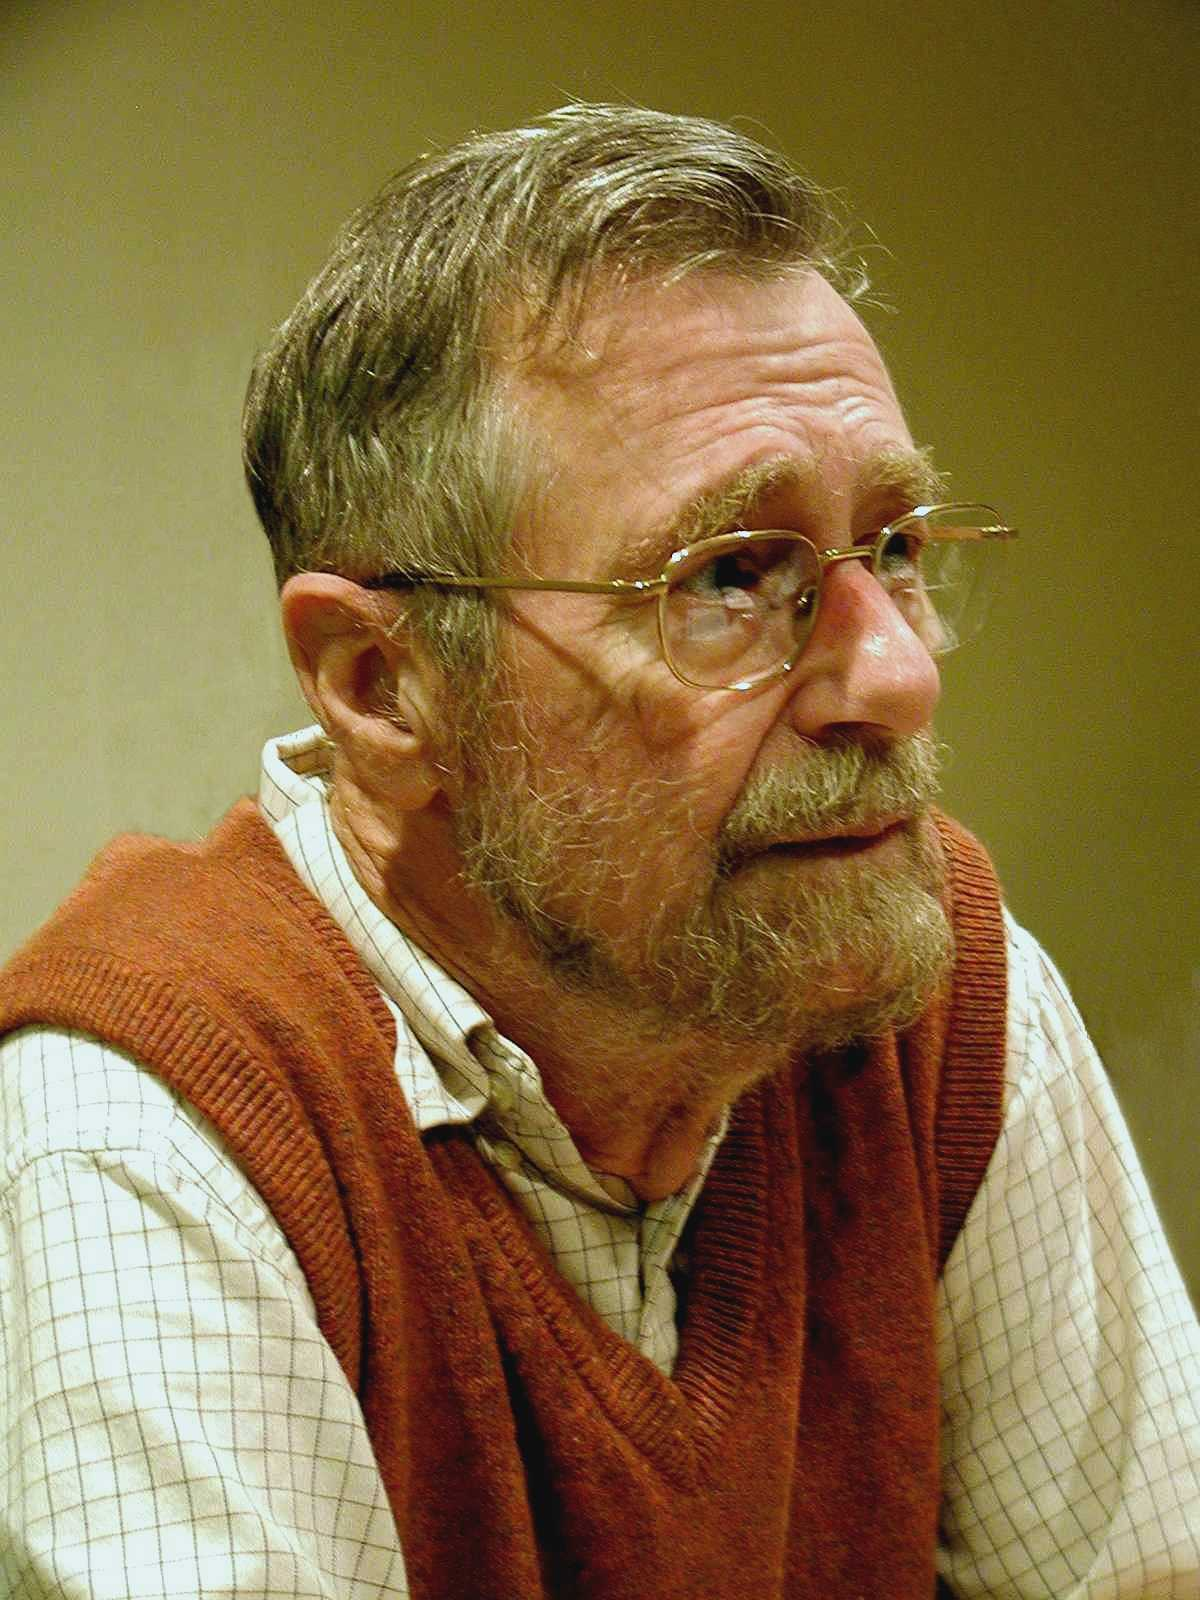
\includegraphics[width=.2\textwidth]{EWD}
			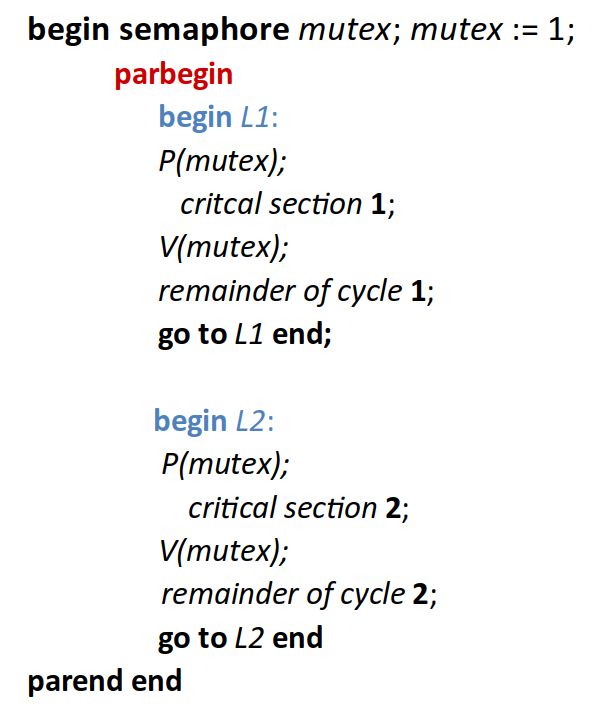
\includegraphics[width=.8\textwidth]{semaphore}
			
			
			
		\end{column}
		
		\begin{column}{.6\textwidth}
			
			%			\large
			Is THE a good system at that time?
			
			Yes
			\begin{itemize}
				\item Performance
				
				\begin{itemize}
					\item 20\% slower than single machine
					\item Short turn‐around time (latency) for short jobs
					\item Benefit from the multi‐programming design choice
					
				\end{itemize}
				
				\item Programmability
				
				\begin{itemize}
					\item virtual BIG memory
					\item Benefit from the VM design choice
					
				\end{itemize}
			
			    \item Reliability
			\end{itemize}	
			
		\end{column}
		
		
	\end{columns}
	
	
\end{frame}
%-------------------------------------------------


\end{document}